%\documentstyle[epsf,twocolumn]{jarticle}       %LaTeX2.09仕様
%\documentclass[twocolumn]{jarticle}     %pLaTeX2e仕様
\documentclass{jarticle}     %pLaTeX2e仕様

%一枚組だったら[twocolumn]関係のとこ消す

\setlength{\topmargin}{-45pt}
%\setlength{\oddsidemargin}{0cm} 
\setlength{\oddsidemargin}{-7.5mm}
%\setlength{\evensidemargin}{0cm} 
\setlength{\textheight}{24.1cm}
%setlength{\textheight}{25cm} 
\setlength{\textwidth}{17.4cm}
%\setlength{\textwidth}{172mm} 
\setlength{\columnsep}{11mm}

\kanjiskip=.07zw plus.5pt minus.5pt

\usepackage{graphicx}
\usepackage[dvipdfmx]{color}
\usepackage{subcaption}
\usepackage{enumerate}
\usepackage{comment}
\usepackage{url}
\usepackage{multirow}
\usepackage{diagbox}
\usepackage{amsmath,amssymb}
\usepackage{mathtools}
\usepackage{wrapfig}


\begin{document}
  \noindent
  \onecolumn
  \hspace{1em}

  \today
  ゼミ資料
  \hfill
  \ \ B3 西村昭賢 

  \vspace{2mm}
  \hrule
  \begin{center}
  {\Large \bf 進捗報告}
  \end{center}
  \hrule
  \vspace{3mm}


\section{今週やったこと}

\begin{quote}
  \begin{itemize}
   \item python でカードゲームの再実装
   \item 実験環境の構築
   \item 簡単な条件下の基礎実験
  \end{itemize}
 \end{quote}

\section{Python で実装したカードゲーム}
 Python だけでカードゲームの対戦を行えるように, Python で簡単なカードゲームを作成した.
 プレイヤーは HP を持ち,カードは攻撃力と HP をそれぞれ持つ用に設定した.
 またカードが敵カードに攻撃する際には,敵カードから攻撃を受けないようにした.
 カードのコスト,それに関するマナコスト,カードに付随する特殊効果などは未実装である.
 実装したコードは \url{https://github.com/1g-hub/Nishimura/tree/main/Sources}

\section{実験環境の構築}
自作ゲームを学習環境として利用する方法として OpenAI Gym を採用した.
OpenAI Gym を採用した理由は 2 つあり, 1 つは OpenAI Gym 用のラッパーや自作環境は多くの人が作成・公開しているためインターネット上に参考になる資料が多くあるため,もう 1 つは OpenAI Gym に対応している強化学習フレームワークが多く自作環境と学習モデル構築部分を分離して作成することができるためである\cite{OpenAI}.
OpenAI Gym を用いて自作環境を作成する際,エージェントが取りうる行動空間,状態空間,報酬の 3 つを定義する必要がある.基礎実験でどのように定義したかは以下の節で示す.
\par
また,強化学習フレームワークとして keras を採用した.
後々細かいチューニングが必要であると思われるが,実験を回す際に簡単にモデルを作成することができるため採用した.


\section{基礎実験}
構築した環境がうまく機能しているかどうか確かめるため,先週のゼミでアドバイスを頂いたように簡単な条件下で実験した.

\subsection{条件}

各プレイヤーについて 3 枚場に出るカードを用意し, Play (手札から場に出す動作), Draw (デッキからカードを引く)といった動作を考慮せず先攻と後攻に分かれて 1 ターンの勝負を行う.学習する対象は先攻のプレイヤーとして,後攻のプレイヤーは先攻プレイヤーの場における最も攻撃力が高いカードを優先的に狙うように設定した.カードの数値はカードゲームでは一般的に先手が有利であることを考慮して適当に定めた.また,各プレイヤーの HP は 20 とした.
条件下におけるカードゲームのイメージを図 \ref{fig:Figure1} に示す.

\begin{figure}[htbp]
  \centering
  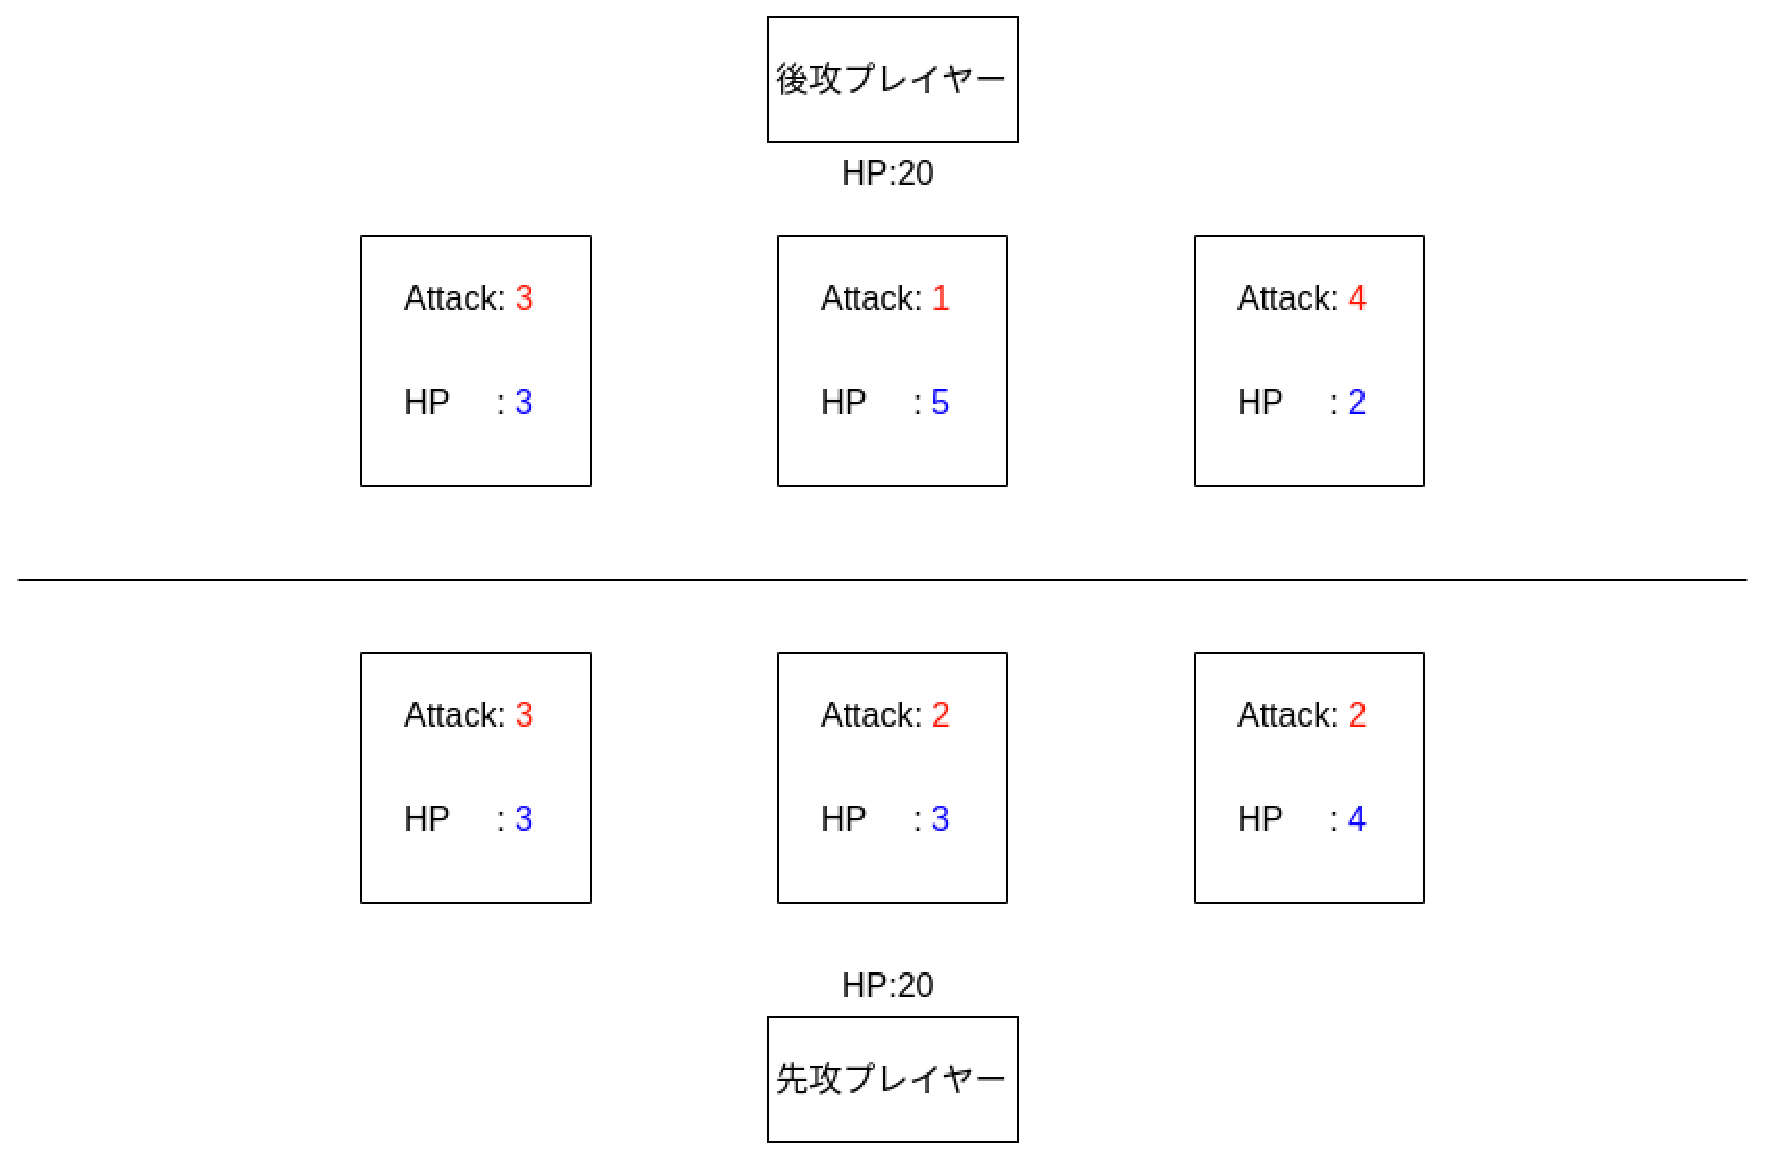
\includegraphics[width=150mm]{assets/Figure1.eps}
  \caption{基礎実験における条件設定のイメージ図}
  \label{fig:Figure1}
\end{figure}

\subsection{自作環境下におけるエージェントの行動空間の定義}
OpenAI Gym では,エージェントの行動を離散値で与えることが多い.そのためにはプレイヤーの行動を数え上げ行動空間を定義する必要がある.本実験では,
\begin{quote}
  \begin{itemize}
   \item プレイヤーのカードが相手プレイヤーを攻撃する・・・ 3 通り
   \item プレイヤーのカードが敵プレイヤーのカードを攻撃する・・・ 3*3 = 9 通り
  \end{itemize}
 \end{quote}
の合計 12 通りと定義して実装した.

\subsection{状態空間の定義}
プレイヤーが観測できる情報は定義により様々に考えられるが本実験では,
\begin{quote}
  \begin{itemize}
   \item プレイヤー 2 名の HP
   \item プレイヤー双方の場に出ているカード 6 枚の攻撃力と HP 
   \item ターン中行動したかどうか(先攻プレイヤーのカードのみ)
  \end{itemize}
 \end{quote}
の合計 17 個のパラメータからなる状態空間を定義して実装した.

\subsection{報酬の定義}
学習における 1 ステップはエージェントの 1 行動に対応している.
報酬の定義として参考文献を参考に以下の式を立てた\cite{reward}.
\begin{equation*}
  \begin{split}
    f(\mathrm{盤面}) = 
    &\alpha*\mathrm{(味方カードの評価値の和)}+\beta*\mathrm{(ターン中に削った敵プレイヤーの体力)}\\
   & - \gamma*\mathrm{(敵カードの評価値の和)} - \delta*\mathrm{(ターン中に削られた自プレイヤーの体力)}\\
    &where \qquad \alpha , \beta , \gamma , \delta \in \mathbb{R}^+
  \end{split}
\end{equation*}
\begin{equation*}
  \quad reward \text{ = }
  \left\{
    \begin{aligned}
        1 \quad &(f(\mathrm{盤面}) \geqq 0) \\
        -1 \quad &(f(\mathrm{盤面}) < 0)
    \end{aligned}
    \right.
\end{equation*}
なお,本実験では $\alpha = 2.0$ , $\beta = 1.5$ , $\gamma = 1.0$ , $\delta = 5.0$ とした.またカードの評価値はカードの攻撃力と残り HP の和と定義している.
上式の $reward$ は 1 エピソード,すなわち両プレイヤーの行動終了後に計算される.
ターン中では,基本は $reward = 0$ とし,同じ行動が続いた時は不適切として $reward = -1.0$ としている.

\subsection{作成したモデル,エージェント}
keras , keras-rl を用いて,ネット上のサンプルコード\cite{DQNcode}を参考に Deep Q Network を実装した.ネットワークの概形を 図\ref{fig:model} に示す.
観測できる環境の次元を入力としてこのモデルを通して行動空間の次元の出力を得る.\par

\begin{wrapfigure}{r}{60mm}
  \centering
  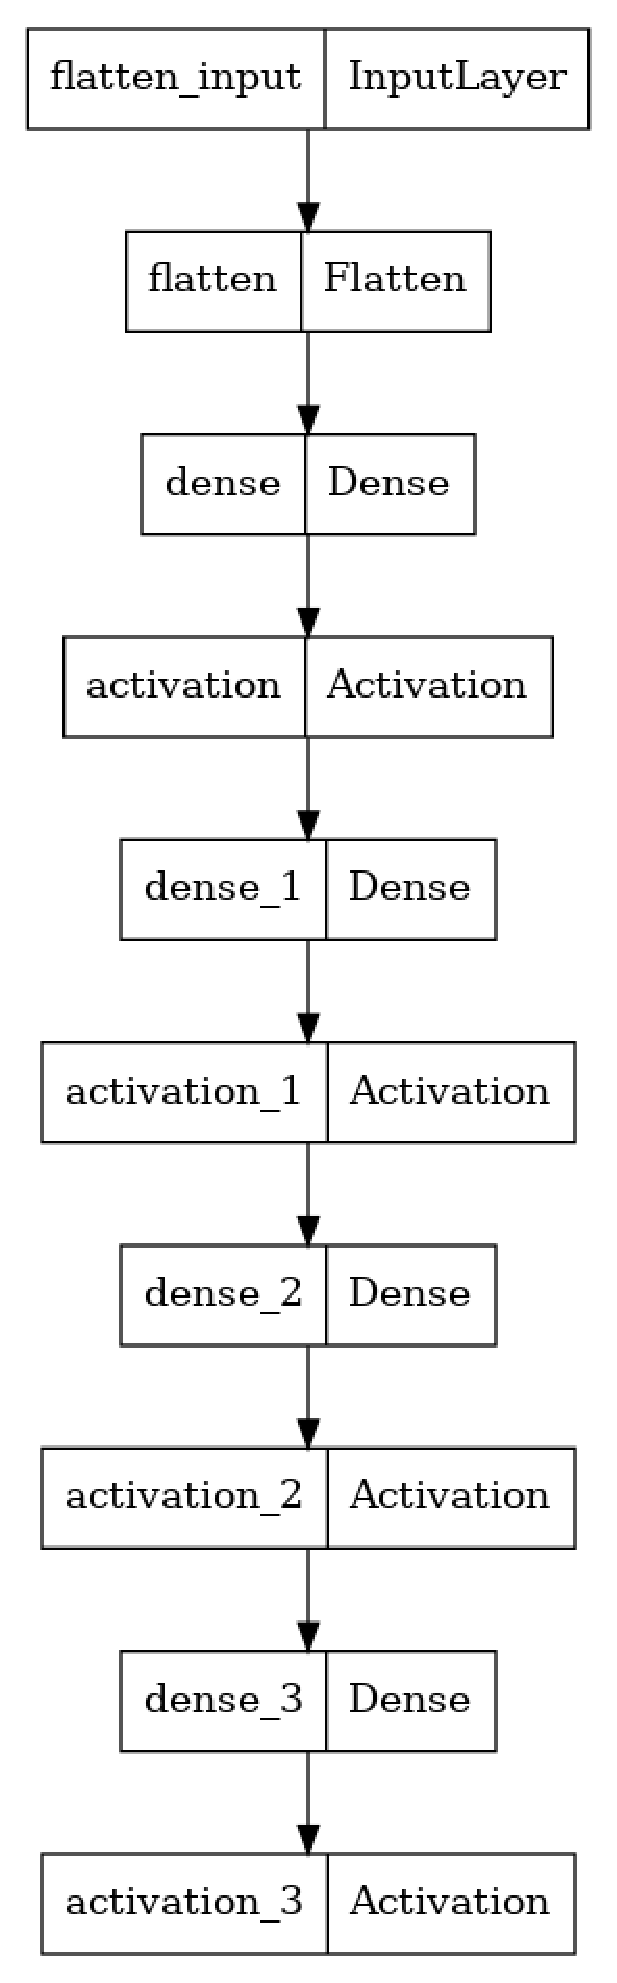
\includegraphics[scale=0.4]{assets/model.eps}
  \caption{モデルの構造}
  \label{fig:model}
\end{wrapfigure}

エージェントの設定として, Exprience Replay のメモリの上限サイズ $limit = 1000000$ ,観測の連結サイズ $window\_length=1$ としている.また,行動方策として $\epsilon$-greedy 法を用いており $\epsilon = 0.1$ としている.最適化関数として Adam を用いており, $learning\_rate = 1e-3$ と設定した.

\subsection{実験結果}
10000 ステップ実験を回した.

図 \ref{fig:graph} は実験において学習過程で 1 エピソードごとのステップ数,報酬を記録したものである.

\begin{figure}[htbp]
  \centering
  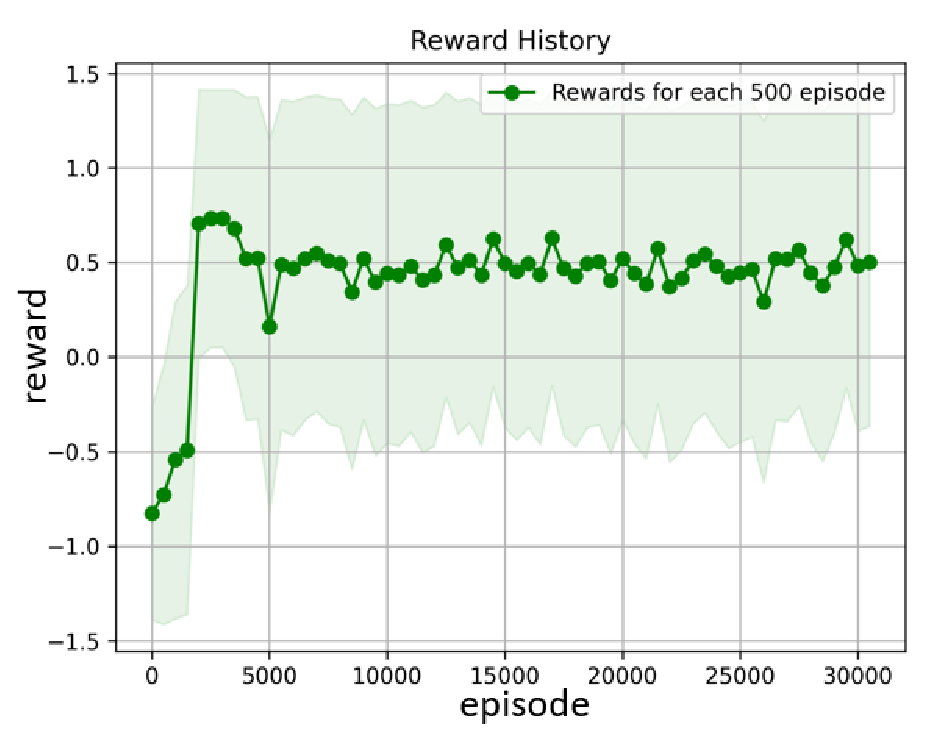
\includegraphics[width=155mm]{assets/graph.eps}
  \caption{ 1 エピソードごとのステップ数,報酬}
  \label{fig:graph}
\end{figure}

また,図 \ref{fig:Log} には学習の後検証を行った際の最後のエピソードにおけるログを示している.
この時,図 \ref{fig:Figure1} において action = [11, 5, 1] となっているが,これは学習によって得られた先攻プレイヤーの行動を意味しており,
 ( Attack , HP ) = ( 2 , 4 ) のカードで敵の ( 4 , 2 ) のカードを攻撃し,( 2 , 3 )のカードで敵の( 3 , 3 )カードを攻撃, ( 3 , 3 ) のカードで敵の ( 3 , 3 ) のカードを攻撃するという行動を意味する.

\subsection{考察}
図3において,今回実装した環境が学習環境として正常に動作していることがわかる.今回の実験設定の場合,先攻プレイヤーの理想的な動作は3枚のカードを最大の報酬を得られるように使うことであり, steps は 3 ,その時の reward は 1 となる.
実際図 \ref{graph} ではエピソードを重ねていくにつれ理想的な値に近づいていっている.初期のエピソードなどの値の絶対値が多い時は,エージェントが探索を優先しいろいろな action を試しており,そのため action の重複が発生し steps の値が大きくなり reward の値が小さくなっていったと考えられる.

一方,実験結果に関しては人間視点では理想的なカードの動かし方とは言えない.
 ( 2 , 3 )のカードで ( 3 , 3 )のカードを攻撃するのは無意味であり,相手プレイヤーに直接攻撃したほうがより高い報酬を得られた.
これはステップの試行回数の少なさ,報酬の定義の仕方に問題があると考えられる.
\begin{figure}[htbp]
  \centering
  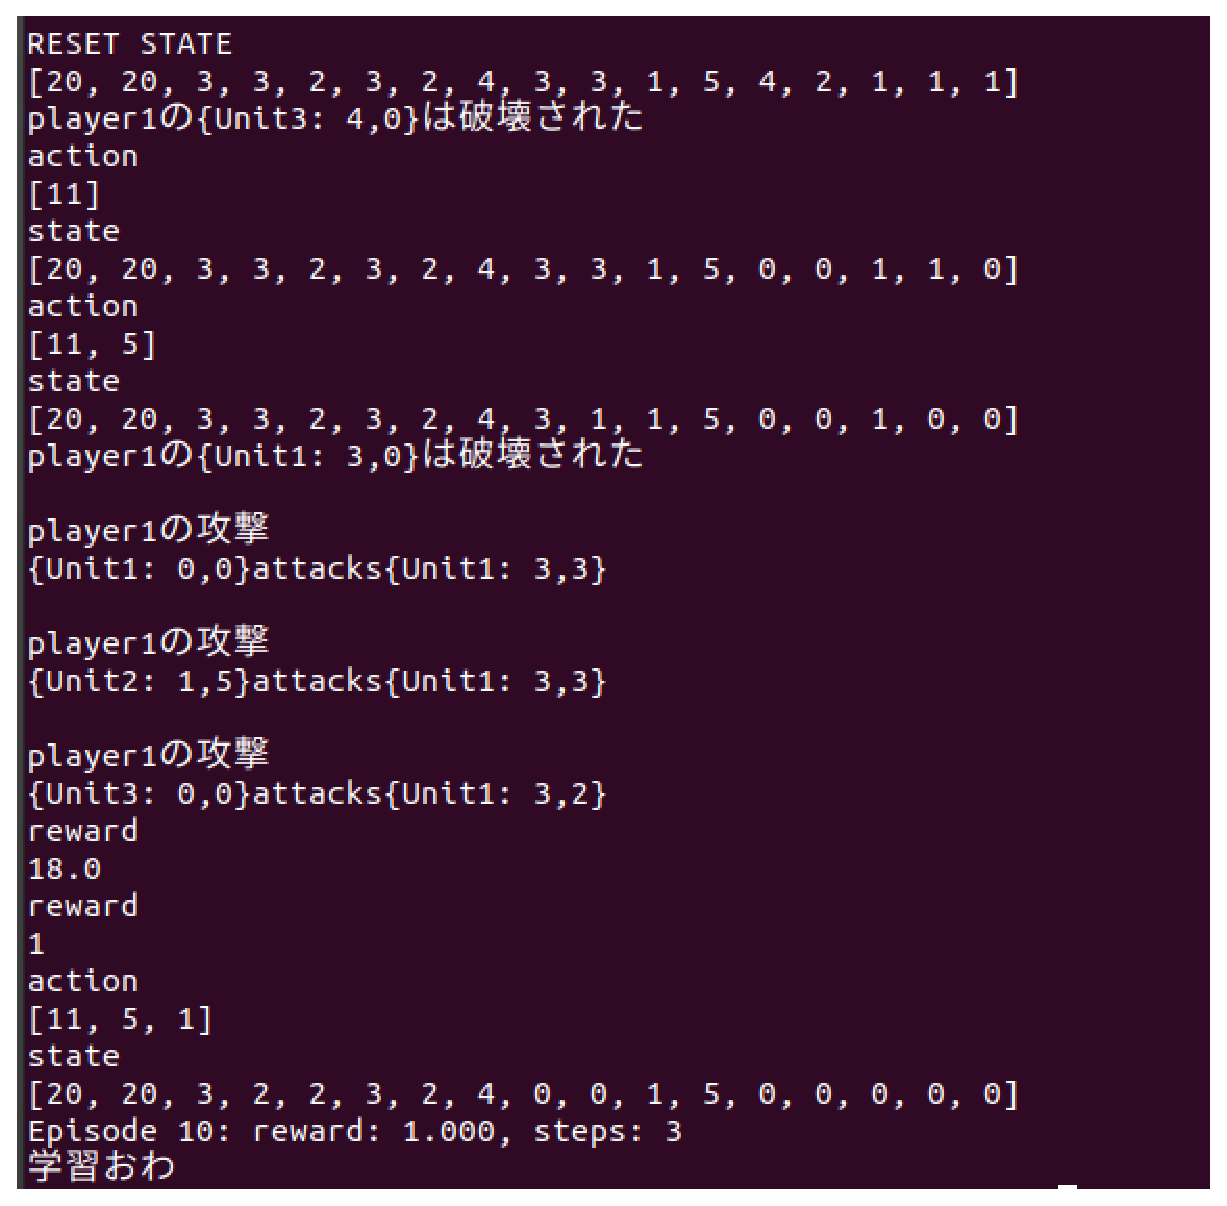
\includegraphics[width=105mm]{assets/Log.eps}
  \caption{検証過程における最後のエピソードのログ}
  \label{fig:Log}
\end{figure}

\section{今後の課題}


\begin{quote}
  \begin{itemize}
   \item 自作の環境の改良
   \par
    今回の実験では, Draw や Play , TurnChange といった動作を考慮せず事前に盤面を設定した.
    このことで4.2節で述べた行動空間の定義を簡単に求めることができた.
    しかし,実際のカードゲームではターンが変わるたびに盤面の状況が変わるため逐一行動空間の次元を求めて環境に適用させなければならない.また,手札などの要素が加わると行動空間の次元が途端に増えるため対処法を考慮,実装する必要がある.\par
    また,実験結果がログとして出てきているが分かりづらいので分かりやすい実験結果の表示を行えるようにしたい.
    \item カードゲーム自体の改良
    \par
    2節で述べたようにシャドウバースやハースストーンに見られるコスト,特殊効果といった要素をまだ実装できていない.必要に応じてやる.
    \item 自動難易度調整の方法検討
    \par
    カードのパラメータを何かしらの結果に基づいて変更すれば良い ? としか思っていないため類似研究などから知識を深めたい.

  \end{itemize}
 \end{quote}

%index.bibはtexファイルと同階層に置く
%ちゃんと\citeしないと表示されない(1敗)
\bibliography{index.bib}
\bibliographystyle{junsrt}

\end{document}